% DRAFT generated as a starting point. Rewrite in my own voice before anyone reads it (see SPEC.md Section 9).
% Passive voice, undergraduate style, as requested.
% Compile from the repo root: pdflatex README.tex
\documentclass[11pt,a4paper]{article}

\usepackage[margin=1in]{geometry}
\usepackage{graphicx}
\usepackage{booktabs}
\usepackage{tabularx}
\usepackage[hidelinks]{hyperref}
\usepackage{listings}
\usepackage{xcolor}
\usepackage{caption}

\graphicspath{{results/figures/}}
\newcommand{\degC}{\ensuremath{^{\circ}}C}

\lstset{basicstyle=\ttfamily\small, backgroundcolor=\color{gray!10},
        frame=single, breaklines=true, columns=fullflexible}

\title{Predicting the LCST of NIPAM copolymers}
\author{}
\date{}

\begin{document}
\maketitle

PNIPAM is dissolved in cold water and becomes cloudy at about 32\,\degC. This
temperature can be shifted by copolymerising NIPAM with a second monomer, and this
effect is used in the smart nanofibers developed in Mitsuhiro Ebara's group at NIMS.
In those fibers, NIPAM is copolymerised with N-hydroxymethylacrylamide (HMAAm) so
that the switch is raised to the mild-hyperthermia range, around 42 to 45\,\degC.

In this project, the question of how well that temperature can be predicted from
the structure of the comonomer and its amount in the chain was studied. Published
LCSTs for NIPAM copolymers were collected, each comonomer was described with a small
number of descriptors, and the model was tested on comonomers that were not seen
during training, including the HMAAm copolymers reported by the Ebara group.

\section*{Main result}

It was found that a ridge regression on four fraction-weighted features (the change
in logP, polar surface area, and H-bond donors of the comonomer relative to NIPAM)
predicted the LCST of held-out comonomers with a mean absolute error of 4.3\,\degC.
For comparison, an error of 8.9\,\degC{} was obtained when 32\,\degC{} was predicted
for every copolymer, and an error of 6.6\,\degC{} was obtained with a straight line
in mole fraction (Figure~\ref{fig:summary}).

For the Ebara group's HMAAm copolymers, all HMAAm rows were removed from training
before the prediction was made. An error of 2.6\,\degC{} was obtained across 7
measurements, and all 7 values were found inside the 90\% prediction interval
(Figure~\ref{fig:ebara}). The predictions were about 3 to 4\,\degC{} too high near
20\,mol\% HMAAm.

No improvement was obtained with the 4215 alvaDesc descriptors. These models appeared
accurate under random cross-validation but failed when new comonomers were predicted.

\begin{figure}[h]
  \centering
  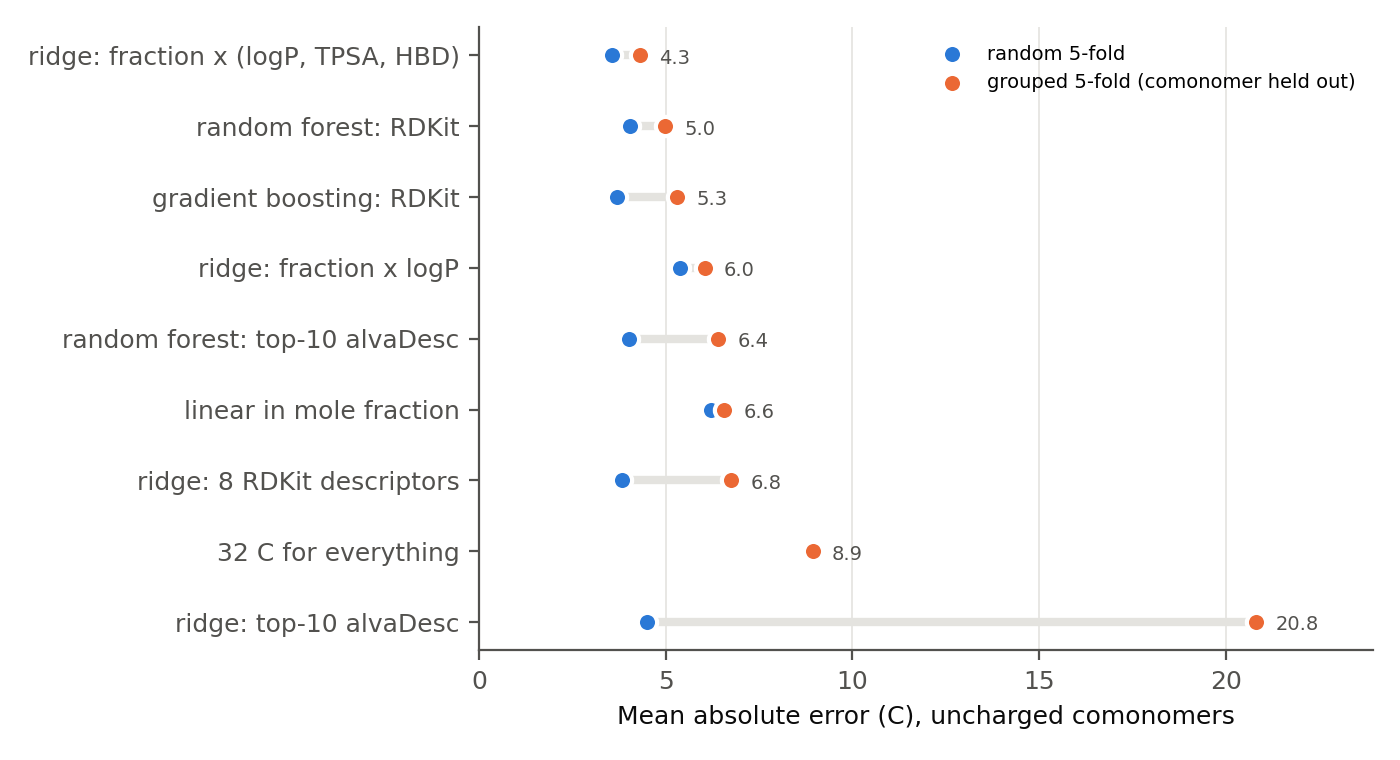
\includegraphics[width=0.85\textwidth]{results_summary.png}
  \caption{Mean absolute error under random 5-fold (blue) and grouped 5-fold
  cross-validation, in which every row of a comonomer is held out together (orange).
  Uncharged comonomers, 103 rows.}
  \label{fig:summary}
\end{figure}

\begin{figure}[h]
  \centering
  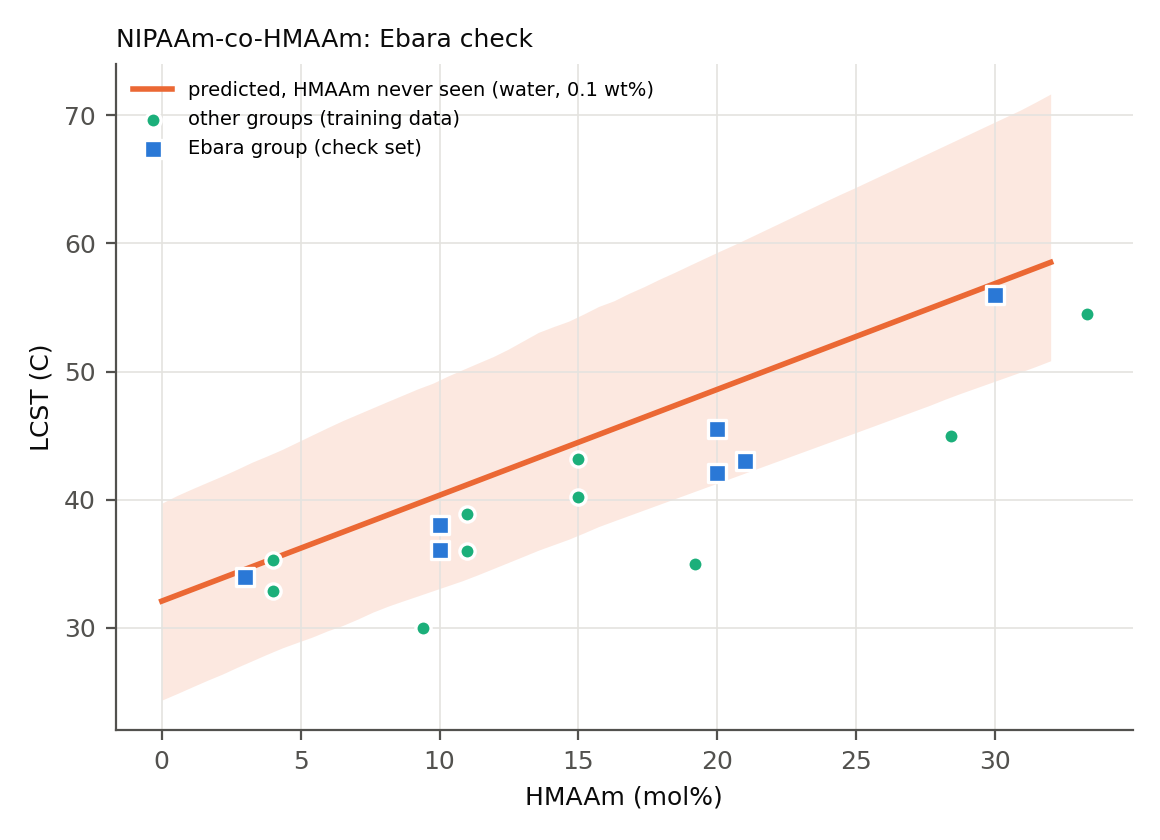
\includegraphics[width=0.62\textwidth]{ebara_check.png}
  \caption{Ebara group HMAAm copolymers (squares) against the prediction of a model
  that was trained without any HMAAm data (line, 90\% interval shaded). Circles are
  HMAAm data from other groups, which were not used for this prediction.}
  \label{fig:ebara}
\end{figure}

\section*{How to run}

Python 3.13 was used (Python 3.11 was specified in the spec but was not available;
the change is recorded in the changelog in \texttt{SPEC.md}).

\begin{lstlisting}[language=bash]
pip install -r requirements.txt
bash run.sh
\end{lstlisting}

The stages 1 to 7 are run in order by \texttt{run.sh}, and the whole analysis is
rebuilt from \texttt{data/raw/} in about 7 minutes. Most of this time is taken by
Stage 4.

\section*{What each stage does}

\begin{small}
\begin{tabularx}{\textwidth}{@{}lX@{}}
\toprule
Script & What is done \\
\midrule
\texttt{s1\_comonomers.py} & the dataset schema is checked; every comonomer SMILES is parsed and drawn \\
\texttt{s2\_descriptors.py} & RDKit descriptors and fraction-weighted features are computed; the alvaDesc export is read \\
\texttt{s3\_clean.py} & missing, constant, near-constant, and correlated descriptors are removed (4226 to 470) \\
\texttt{s4\_model.py} & baselines, ridge, random forest, and boosting are trained under random 5-fold, grouped 5-fold, and leave-one-comonomer-out validation \\
\texttt{s5\_trends.py} & the logP trend at fixed fraction, the composition series, and the coefficients are examined \\
\texttt{s6\_ebara\_predict.py} & the Ebara HMAAm check is run with HMAAm held out; new copolymers are predicted with an applicability-domain check \\
\texttt{s7\_summary\_figures.py} & the summary and dataset-overview figures are drawn \\
\bottomrule
\end{tabularx}
\end{small}

\section*{Folder guide}

\begin{lstlisting}
data/raw/          lcst.csv (the dataset), alvadesc_export.txt (the raw descriptor export)
data/processed/    comonomers, descriptors, model table, cleaned features
data/sources.md    all sources, what was taken from each, and what was left out and why
data/pdfs/         paper PDFs used for extraction (git-ignored, not included in the repo)
results/           metrics, predictions, trend tables, figures/
notes/             research_note.tex (and .md)
SPEC.md            the spec that was followed, and the changelog
\end{lstlisting}

\section*{Notes on the data}

\begin{itemize}
  \item There are 113 training rows from 22 sources, covering 22 comonomers and 16
  PNIPAM reference rows. A further 7 rows from four Ebara group papers are kept in the
  same file with \texttt{role = ebara\_check} and were not used for training.
  \item Most rows were taken from tables. 9 rows were read from figures, with an
  accuracy of about 1\,\degC.
  \item 19 rows are values that were compiled from the literature in another paper
  (Hayakawa et al.\ 2023, ESI). The measurement method, and whether the fraction refers
  to the feed or the measured composition, are not given there, so these rows are
  marked with a \texttt{secondary} note.
  \item LCST is measured in different ways in different papers (50\% transmittance,
  first visible turbidity, absorbance thresholds, DSC). The method was recorded for
  every row. This adds a few degrees of noise that cannot be removed by the model.
  \item The LCST of charged comonomers (acrylic acid and two amine monomers) changes
  with pH, so these were left out of the headline numbers. Results with them included
  are given in \texttt{metrics.csv} under \texttt{subset = all}.
\end{itemize}

\section*{Known limitations}

\begin{itemize}
  \item 22 comonomers is a small number, and 18 of them were taken from a single paper each.
  \item The same Crippen logP is given to N-n-propylacrylamide and NIPAM, although the
  homopolymer of N-n-propylacrylamide switches about 10\,\degC{} lower. This kind of
  difference is not captured by simple 2D descriptors.
  \item A negative coefficient was obtained for the TPSA term. Because this term is
  strongly correlated with the logP term ($r = -0.74$), the individual coefficients
  should not be interpreted as separate physical effects.
\end{itemize}

\end{document}
